\documentclass[11pt]{article}
\usepackage[spanish, es-tabla]{babel}
\usepackage{fontspec}
\usepackage{listings}
\usepackage{graphicx}
\graphicspath{{./img/}}

\usepackage[paper=portrait, pagesize]{typearea}
\usepackage{titlepic}

% Listas
\usepackage{amssymb}
\usepackage{enumitem}
\renewcommand{\labelitemi}{$\bullet$}
%%% Tablas
\usepackage{longtable}
\usepackage{tabularx}
\usepackage{float}
\usepackage{adjustbox}
\usepackage{booktabs}
\usepackage{multirow}
\usepackage{url}
\renewcommand{\arraystretch}{1.7}

\begin{document}

\begin{titlepage}
\centering
\vspace{4.5cm}
{\scshape\LARGE Metodología Ágil:\\ Feature Driven Development\par}
\vspace{1.5cm}


\vspace{3cm}
{\scshape\large \par}
\vspace{1cm}

{Miguel Albertí Pons\\
Sofía Almeida Bruno\\
Pedro Manuel Flores Crespo\\
María Victoria Granados Pozo\\
Lidia Martín Chica
\par}

\end{titlepage}
%\cite{SeminarioMunich}

\thispagestyle{empty}
\tableofcontents

\newpage

%%%%%%%%%%%%%%%%%%%%%%%%%%%%%%%%%%%%%%%%%%%%%%%%%%%%%%%%%
%%%% BIBLIOGRAFÍA
%%%%%%%%%%%%%%%%%%%%%%%%%%%%%%%%%%%%%%%%%%%%%%%%%%%%%%%%%
\section{Introducción}

Feature-Driven Development (FDD) es una metodología ágil propuesta por Jeff De Luca y Peter Coad en 1997. FDD no cubre todo el proceso de desarrollo de software, se enfoca en las fases de diseño e implementación. Se caracteriza por tener muchas iteraciones muy cortas, prestando atención a la calidad, con entregas frecuentes de trabajo tangible en todos los pasos.\\

FDD está enfocada en el desarrollo de las características (similares a las historias de usuario de Scrum), utiliza como criterio en la planificación el valor que estas tienen para el cliente.\\

FDD es una metodología adecuada para equipos más grandes, con más personas que aquellos donde normalmente se utilizan otras metodologias como SCRUM, y proyectos más complejos. FDD ve necesaria la figura del jefe de proyecto y una fase donde se define la arquitectura.\\

En este documento veramos los 5 procesos que hay que seguir para aplicar FDD, las ventajas de esta metodología y los roles con sus respectivas responsabilidades.

\section{Procesos}

La metodología FDD consta de cinco fases secuenciales en su proceso durante las cuales se diseña e implementa el sistema. Se comienza creando un modelo del dominio con la colaboración de expertos en el tema. Usando esta información y la obtenida en las actividades de requisitos se crea una lista de características. Entonces se establece un plan y se asignan responsabilidades, los equipos van desarrollando pequeños grupos de características en menos de dos semanas. En la Figura \ref{fig:proc} observamos los procesos de la metodología FDD, se itera en la parte de diseñar e implementar las características.

\begin{figure}[H]
    \centering
    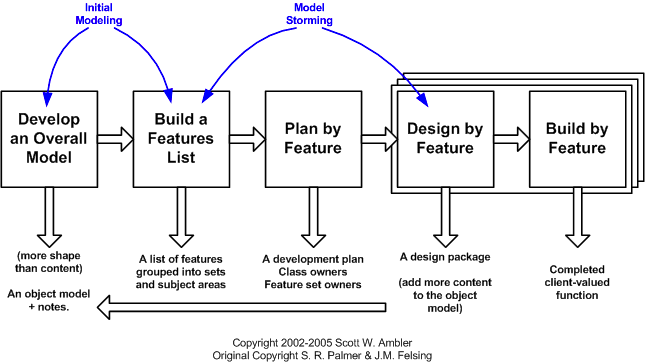
\includegraphics[width=0.9\textwidth]{lifecycle}
    \caption{Procesos en un proyecto FDD.}
    \label{fig:proc}
\end{figure}

\subsection{Desarrollar el modelo global (\textit{Develop overall model})}
En esta primera etapa los miembros del equipo de desarrollo trabajan juntos para construir un modelo del problema del dominio. Su objetivo es proponer el modelo para el área de dominio. El modelado FDD es una actividad interfuncional, iterativa y colaborativa. Los miembros del equipo (desarrollo, expertos en dominios y programadores principales) trabajan juntos para componer un modelo para el área de dominio y son guiados por un Arquitecto Jefe (\textit{Chief Arquitect}). La idea es tener diferentes equipos proponiendo diferentes modelos y luego, después de ser revisados, seleccionar uno de los modelos propuestos o una combinación de modelos y que se convierta en el modelo para esa área de dominio. A medida que se desarrolle el modelo y el equipo aprenda, se agregarán detalles. Esto ayuda al equipo a tener una visión general clara de todo el proyecto, así como una comunicación sólida. Las tareas llevadas a cabo en esta etapa se resumen en la Tabla \ref{fig:DOM}. 

\begin{table}[H]
  \centering
\begin{tabular}{ |p{6cm}|p{6cm}|  }
	\hline
	Tarea & Responsables \\
	\hline
	Formación del
	\textit{Model Team}  &    \textit{Project
		Manager}\\
	
	\textit{Domain Walkthrough}  &    \textit{Modeling Team}\\
	
	Estudio de los documentos     &    \textit{Modeling Team}\\
	
	Construcción de una \textit{Feature List informal}  &    \textit{Chief Arquitect}, \textit{Chief} y \textit{Programmers}\\
	Desarrollo del \textit{Modelo de Tareas} & \textit{Modeling Team} dividido en pequeños grupos\\
	Desarrollo del \textit{Modelo Global}  &  \textit{Chief Arquitect} y \textit{Modeling Team}\\
	Registro de alternativas    & \textit{Chief Arquitect}, \textit{Chief} y \textit{Programmers}\\
	\hline
\end{tabular}
\caption{Tareas etapa del desarrollo del modelo global.}\label{fig:DOM}
\end{table}

\subsection {Construir lista de características (\textit{Build Feature List})}

Esta etapa recibe como entrada el modelo de objetos y los requerimientos (\textit{feature list informal}) obtenidos en la etapa anterior. Estos son agrupados según el área de dominio. Cada grupo se denomina \textit{Major List Sets}. Esta lista, a su vez, es dividida en otros subconjuntos según la funcionalidad. Posteriormente, cada característica o funcionalidad es priorizada y por último aquellas más complejas son divididas en otras más pequeñas. Esta etapa nos aporta como salida la \textit{Feature List} que es revisada por los usuarios para su aprobación y validación. Las tareas llevadas a cabo en esta etapa se resumen en la Tabla \ref{fig:BFL}. \\

\begin{table}[H]
  \centering
\begin{tabular}{ |p{6cm}|p{6cm}|  }
	\hline
	Tarea & Responsables \\
	\hline
	Formación del
	\textit{Feature-List Team}  &    \textit{Project
		Manager} y 
	\textit{	Development
		Manager}\\
	Identificación de funcionalidades y formación del \textit{Feature Set}  & \textit{Feature-List Team}\\
	Priorización de las funcionalidades &  \textit{Feature-List Team}\\
	División de las funcionalidades complejas    & \textit{Feature-List Team}\\
	\hline
\end{tabular}
\caption{Tareas etapa de construcción de la lista de características.}\label{fig:BFL}
\end{table}

\subsection{Planificado por características (\textit{Plan by feature})}
Este paso gira entorno a la planificación, esto es, el orden en el que se van a implementar las características, la forma de hacerlo y quién las va implementar, asignando tareas a los desarrolladores.
Durante la planificación consideramos diferentes aspectos como riesgos, complejidad, dependiencias, la carga de trabajo, etc, para evitar que surjan problemas complejos a posteriori.

En esta etapa se incluye la creación de un plan de alto nivel, en el cual la \textit{features list} se ordena en base a la prioridad y a la dependencia entre cada característica. A continuación, el gestor del proyecto, el desarrollador y el programador jefe establecen hitos y diseñan un cronograma de diseño y construcción.

Finalmente se realiza una verificación del plan, por parte del gestor del desarrollo y del jefe del producto, teniendo en cuenta la opinión de todos lo miembros del equipo. La salida es un plan de desarrollo incluyendo la fecha de finalización, para cada conjunto de características y para cada característica indicar el programador jefe asignado, y las fechas de inicio y fin. Por último, para cada clase indicar el correspondiente programador de la clase.


\subsection{Diseñando por características (\textit{Design by feature})}
Esta etapa y la siguiente se realizan de forma iterativa, cada iteración debería durar entre unos pocos días y un máximo de dos semanas. Puede haber varios equipos de características trabajando simultáneamente en el diseño e implementación de su propio conjunto de características. 

En esta etapa el \textit{chief programmer}, aprovechando el conocimiento obtenido en las primeras etapas del proceso, selecciona las siguientes características a realizar entre las que tenga en su lista de características asignadas. A continuación, organiza los equipos de características identificando los \textit{class owners} (desarrolladores) que estarán involucrados en el desarrollo de las características seleccionadas y contacta con los expertos de dominio si es necesario. Parte del grupo puede trabajar en el diseño técnico mientras otros trabajan en la infraestructura, escribiendo clases, determinando los métodos y realizando los diagramas de secuencia correspondientes que el \textit{chief Programmer} añadirá al modelo global. Asimismo, cada \textit{class owner} actualizará la descripción de sus clases en base al diagrama de secuencia (añadiendo parámetros, tipos de retorno, mensajes enviados, etc).

Antes de pasar a la siguiente fase todo el equipo revisará y verificará el diseño.

Como salida de esta etapa se debe obtener: el diagrama de secuencia detallado, diagrama de clases actualizado, descripción de clases y métodos, notas del equipo significativas para el diseño.

\subsection{(\textit{Build by feature})}



\section{Comparación con otros métodos}
FDD es una mezcla entre eXtremeProgramming y Scrum, añadiendo técnicas de Domain Driven Design\footnote{Diseño guiado por el dominio (DDD), es un enfoque para el desarrollo de software con necesidades complejas mediante una conexión entre la implementación y los conceptos del modelo y núcleo del negocio. El DDD no es una tecnología ni una metodología, este provee una estructura de prácticas y terminologías para tomar decisiones de diseño.}. A continuación se muestran los puntos en los que se diferencia FDD con XP y Scrum.


\subsection*{Comunicación}
Los métodos ágiles se centran bastante en la comunicación entre los mienbros del equipo y el resto de personas interesadas en el proyecto.

En XP y Scrum la documentación también es importante.

\subsection*{Centro de usuarios}

El \textit{software} debe diseñarse y desarrollarse por un centro de usuarios. Con XP por ejemplo, se necesita la participación de los clientes durante el desarrollo así como iteraciones cortas, al final de las cuales el cliente puede probar el \textit{software}.

\subsection*{Duración del sprint}
Lo normal es usar iteraciones cortas, por ejemplo entre 2 y 10 días. A diferencia de Scrum que dura entre 2 y 4 semanas y XP que puede durar 6 semanas.

\subsection*{Reuniones}
Tanto la comunicación como las reuniones son importantes en los métodos ágiles. Con Srum y XP hay reuniones diarias donde participan todos los miembros del equipo y comentan en que punto del proyecto se encuentran. 

En FDD es un poco diferente por que en general la información se comunica mediante la documentación.

\subsection*{Tamaño del proyecto}

Dependiendo de cada proyecto hay que elegir que método ágil utilizar. Para proyectos cortos y no muy complejos, habría que elegir XP, mientra que para proyectos más complejos y largos es mejor Scrum y FDD.


\section{Ventajas}
FDD minimiza la complejidad del sistema por lo que es una excelente solución para proyectos grandes y complejos, dando al equipo la capacidad de dividir el problema en problemas más pequeños que se pueden resolver en menos tiempo.

La comprensión más profunda del sistema de software reduce el riesgo de encontrar problemas durante el desarrollo.

La mayoría de los procesos requieren un flujo de comunicación constante y la realización frecuente de los informes de progreso en casi cualquier nivel del desarrollo del proyecto, permiten al equipo realizar un seguimiento del progreso y los resultados. Además, FDD permite que los miembros del equipo se comuniquen más fácilmente al tiempo que fomenta la creatividad e innovación del equipo.

El hecho de que en FDD se realicen compilaciones regulares garantiza que se puedan identificar fácilmente errores en el código y permite mantener el proyecto actualizado regularmente, identificar cualquier error y que se pueda mostrar al cliente en cualquier momento. 

En FDD se maximiza la calidad ya que el concepto de calidad no solo incluye la prueba del código, sino que también incluye estándares de codificación, auditorías de medición y métricas en el código.

\section{Roles y responsabilidades}

Los proyectos están formados por personas, procesos y tecnología. En esta sección describiremos cómo se organizan los participantes en un proyecto FDD.Esta metodología clasifica sus roles en tres categorías: clave, de apoyo y adicionales. Un miembro de un equipo puede tomar diferentes roles y un rol se puede compartir entre varias personas.\\

A continuación se exponen los seis roles clave junto con sus tareas y responsabilidades:
\begin{itemize}
\item \textit{Project Manager}. Es el líder administrativo y financiero del proyecto. Una de sus tareas es proteger al equipo de distracciones externas y permitir que el equipo trabaje en las condiciones apropiadas. Es responsable de señalar el progreso, manejar los presupuestos, buscar la plantilla, gestionar el equipo, espacio y recursos. Es el que tiene la última palabra sobre el alcance, planificación y personal del proyecto.
\item \textit{Chief Architect}. El jefe de diseño es responsable del diseño global del sistema y de llevar a cabo las sesiones de diseño del sistema con el equipo. Asimismo, toma todas las decisiones finales en los asuntos de diseño. Este puesto requiere de habilidades técnicas y de modelado además de capacidad de asesoramiento. Si es necesario, este rol se puede dividir entre arquitecto del dominio (\textit{Domain Architect}) y arquitecto técnico (\textit{Tecnical Arquitect}).
\item \textit{Development Manager}. Es el responsable de liderar las actividades de desarrollo diarias y resolver los problemas que ocurran entre los miembros del equipo. Es el encargado de resolver los conflictos por los recursos cuando cuando los \textit{Chief Programmers} no consigan ponerse de acuerdo. Este rol se puede combinar con el de \textit{chief architect} o \textit{project manager}.
\item \textit{Chief Programmer}. Es un programador con cierta experiencia ya que ha pasado por todo el proceso de desarrollo varias veces. Se encarga del análisis de requisitos a un alto nivel, de actividades relacionadas con el diseño y de la dirección de equipos pequeños (3 a 6 programadores) para el análisis, diseño y desarrollo de nuevas funcionalidades. También escoge las funcionalidades a desarrollar de la lista, identifica las clases y el \textit{Class Owner} que se necesita en el equipo para la
iteración. Con la ayuda de otros \textit{Chief Programmers} resuelve problemas técnicos y de recursos, y sigue el progreso
del equipo.
\item \textit{Class Owner}. Trabaja bajo la dirección del \textit{Chief Programmer} en tareas de diseño, programación, pruebas y documentación. Es el responsable de las clases que se asignaron y participa en la decisión de qué clase será incluida en la lista de características de la próxima iteración.
\item \textit{Domain Expert}. Son usuarios, patrocinadores, analistas o una mezcla de ellos. Son los que tienen el conocimiento base acerca del software que se está desarrollando y por ello su participación es crítica para el éxito del sistema.
\end{itemize}

Entre los roles de apoyo de FDD se incluyen:

\begin{itemize}
\item \textit{Domain Manager}. Lidera a los expertos en el dominio y resuelve sus diferencias de opinión respecto a los requisitos del sistema.
\item \textit{Release Manager}. Controla la evolución del proceso asegurándose de que los \textit{chief programmers} informen sobre su progreso semanalmente, revisando sus informes y teniendo reuniones cortas con ellos. Entonces informará directamente al \textit{project manager}.
\item \textit{Language Lawyer/Guru}. Es un miembro del equipo responsable de tener un amplio conocimiento sobre un lenguaje o tecnología concreta. Esta papel tiene más importancia cuando el equipo se enfrenta a una nueva tecnología.
\item \textit{Build Engineer}. Es el responsable de configurar, mantener y llevar a cabo el proceso de producción incluyendo el mantenimiento de las versiones y publicación de la documentación.
\item \textit{Toolsmith}. Construye herramientas específicas para el desarrollo, conversión de datos y realización de pruebas. Puede trabajar en la preparación y mantenimiento tanto de bases de datos como de páginas web destinadas al proyecto.
\item \textit{System Administrator}. Configura, administra y repara los servidores, equipos de trabajo, desarrollo y pruebas utilizados. 
\end{itemize}

De forma adicional se tienen los siguientes roles:

\begin{itemize}
\item \textit{Tester}. Se encargan de verificar de forma independiente que el sistema cumple los requisitos del usuario y que realiza esas funciones de la manera adecuada. Puede ser una persona independiente o no del equipo del proyecto.
\item \textit{Deployer}. Convierte la información existente al formato requerido por el sistema y participa en el despliegue físico de los nuevos productos. 
\item \textit{Technical Writer}. Escribe la documentación para los usuarios.

\end{itemize}

\section{Prácticas}
% Sadhna Goyal. Major seminar on feature driven development. In Technical University
Las prácticas más usadas en FDD son:
\begin{enumerate}
\item \textit{Domain Object Modeling}: Consiste en construir diagramas de clases que representan los objetos más significativos dentro de un problema y las relaciones entre ellos. Es una forma de descomposición de objetos. El diseño e implementación de cada objeto o la clase identificada en el modelo es un problema menor para resolver. Una técnica utilizada dentro de esta práctica es \textit{UML in color}. Básicamente, consiste en que las clases se clasifican en diferentes categorías y cada categoría lleva asociada un color. Por ejemplo, el amarillo se usa para clases que representan algún rol (persona u organización) o el  azul para aquellas que guardan la información sobre el objeto que representan.
\item \textit{Developing by Feature}: las funciones que son demasiado complicadas se descomponen en otras más pequeñas hasta tener subproblemas que representen una sola característica.
\item \textit{Class (Code) Ownership}: cada persona o rol es el responsable de sus clases o código implementado.
\item \textit{Feature Teams}: cada característica detectada puede necesitar más de una clase y en consecuencia varios \textit{class owners} por lo que el dueño de cada característica es el encargado de coordinar el trabajo de estos programadores.
\item  \textit{Inspections}: aplicar las técnicas de detección de fallos más conocidas y aprovechar las oportunidades que proporcionan para promover buenas prácticas de desarrollo.
\item  \textit{Regular Build Schedule }: regularmente se debe tomar todo el código desarrollado y construir el sistema completo para asegurarnos que siempre una versión funcional.
\item  \textit{Configuration Management}: sirve para identificar las últimas versiones de los archivos completados y proporciona un seguimiento de todos los artefactos usados.
\item \textit{Progress Reporting}: a lo largo de todo el proyecto realizar informes sencillos que contengan el progreso realizado para informar a todos los roles dentro y fuera del proyecto.
\end{enumerate}

\newpage
\section{Bibliografía}
\nocite{*}
\bibliographystyle{plain}
\bibliography{referencias.bib}
%[type=inbook,heading=subbibliography,title={Libros}]
%TODO: Añadirlo a la bibliografía https://es.wikipedia.org/wiki/Dise%C3%B1o_guiado_por_el_dominio

\end{document}
